%!TEX root = ../TAMUTemplate.tex
%%%%%%%%%%%%%%%%%%%%%%%%%%%%%%%%%%%%%%%%%%%%%%%%%%%
%
%  New template code for TAMU Theses and Dissertations starting Fall 2016.
%
%  Author: Sean Zachary Roberson
%	 Version 3.16.09
%  Last updated 9/12/2016
%
%%%%%%%%%%%%%%%%%%%%%%%%%%%%%%%%%%%%%%%%%%%%%%%%%%%

%%%%%%%%%%%%%%%%%%%%%%%%%%%%%%%%%%%%%%%%%%%%%%%%%%%%%%%%%%%%%%%%%%%%%%%
%%%                           SECTION II
%%%%%%%%%%%%%%%%%%%%%%%%%%%%%%%%%%%%%%%%%%%%%%%%%%%%%%%%%%%%%%%%%%%%%%


\chapter{\uppercase {The LHC and CMS Detector}}

\section{The Large Hadron Collider}

The Large Hadron Collider (LHC) \cite{Breskin:1244506} is, in many people's estimation, the largest and most complex machine ever built by humanity. The main accelerator at the European Organization for Nuclear Research (CERN), the LHC is located both in France and Switzerland due to its enormous size (Fig.~\ref{fig:LHC_schematic}). It was built between 1998 and 2008 and installed in the $26.7\unit{km}$ tunnel dug for its predecessor, the Large Electron-Positron Collider (LEP), which is located between $50\unit{m}$ and $170\unit{m}$ underground. It is the highest energy collider in the world, eclipsing the previous record holder, the Tevatron at Fermilab in Batavia, IL. The following section is a description of the LHC and CERN accelerator complex based on \cite{LHCmachine} and \cite{Breskin:1244506}.

\begin{figure}[!hbt]
	\centering
	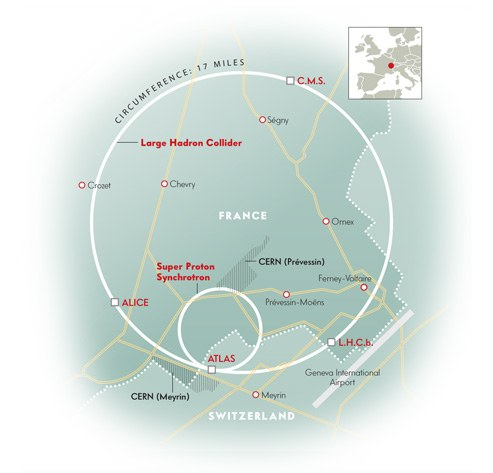
\includegraphics[width=0.95\textwidth]{\figpath/Chapter2/LHC_schematic.jpg}
	\caption{Overhead view of CERN and its main experiments, CMS; ATLAS; LHCb; and ALICE, as well as two of the larger accelerators, the LHC and SPS. The schematic is overlaid on a map of Switzerland and France~\cite{LHC-schematic}.}
	\label{fig:LHC_schematic}
\end{figure}

The LHC provides beams for four main experiments located along its beam line (Fig.~\ref{fig:LHC_schematic}):
\begin{itemize}
	\item The CMS (Compact Muon Solenoid)~\cite{Chatrchyan:2008aa} and ATLAS (A Toroidal LHC ApparatuS)~\cite{1748-0221-3-08-S08003} experiments are both general purpose detectors. Their goals include precision measurements to test the Standard Model and searches for new physics, including the Higgs boson.
	\item LHCb (Large Hadron Collider beauty)~\cite{Alves:2008zz} was designed to do precision measurements of CP-violation and the physics of B-mesons.
	\item ALICE (A Large Ion Collider Experiment)~\cite{Aamodt:2008zz} studies heavy ion collisions.
\end{itemize}

The LHC was designed to collide two beams of protons (pp), heavy ions (PbPb), or a combination of the two (pPb) at specific interaction points around the beam line. For the purposes of this thesis we will only cover proton-proton collisions from this point forward. The protons come from a single bottle of hydrogen gas, which is then disassociated and stripped of electrons to form a proton beam. Interestingly, only $1\unit{ng}$ of hydrogen is required per day in order to form the LHC beams. The protons next travel through the Linac2 machine where they form bunched by radio frequency (RF) electromagnetic fields and are accelerated to $50\unit{MeV}$. This chain continues through the Proton Synchroton Booster (PSB), the Proton Synchrotron (PS), and the Super Proton Synchrotron (SPS) where the protons are accelerated to $1.4\unit{GeV}$, $26\unit{GeV}$, and $450\unit{GeV}$ respectively (Fig.~\ref{fig:CERN_accelerators}).

\begin{sidewaysfigure}[!hbt]
	\centering
	\begin{subfigure}[t]{0.4655\textwidth}
		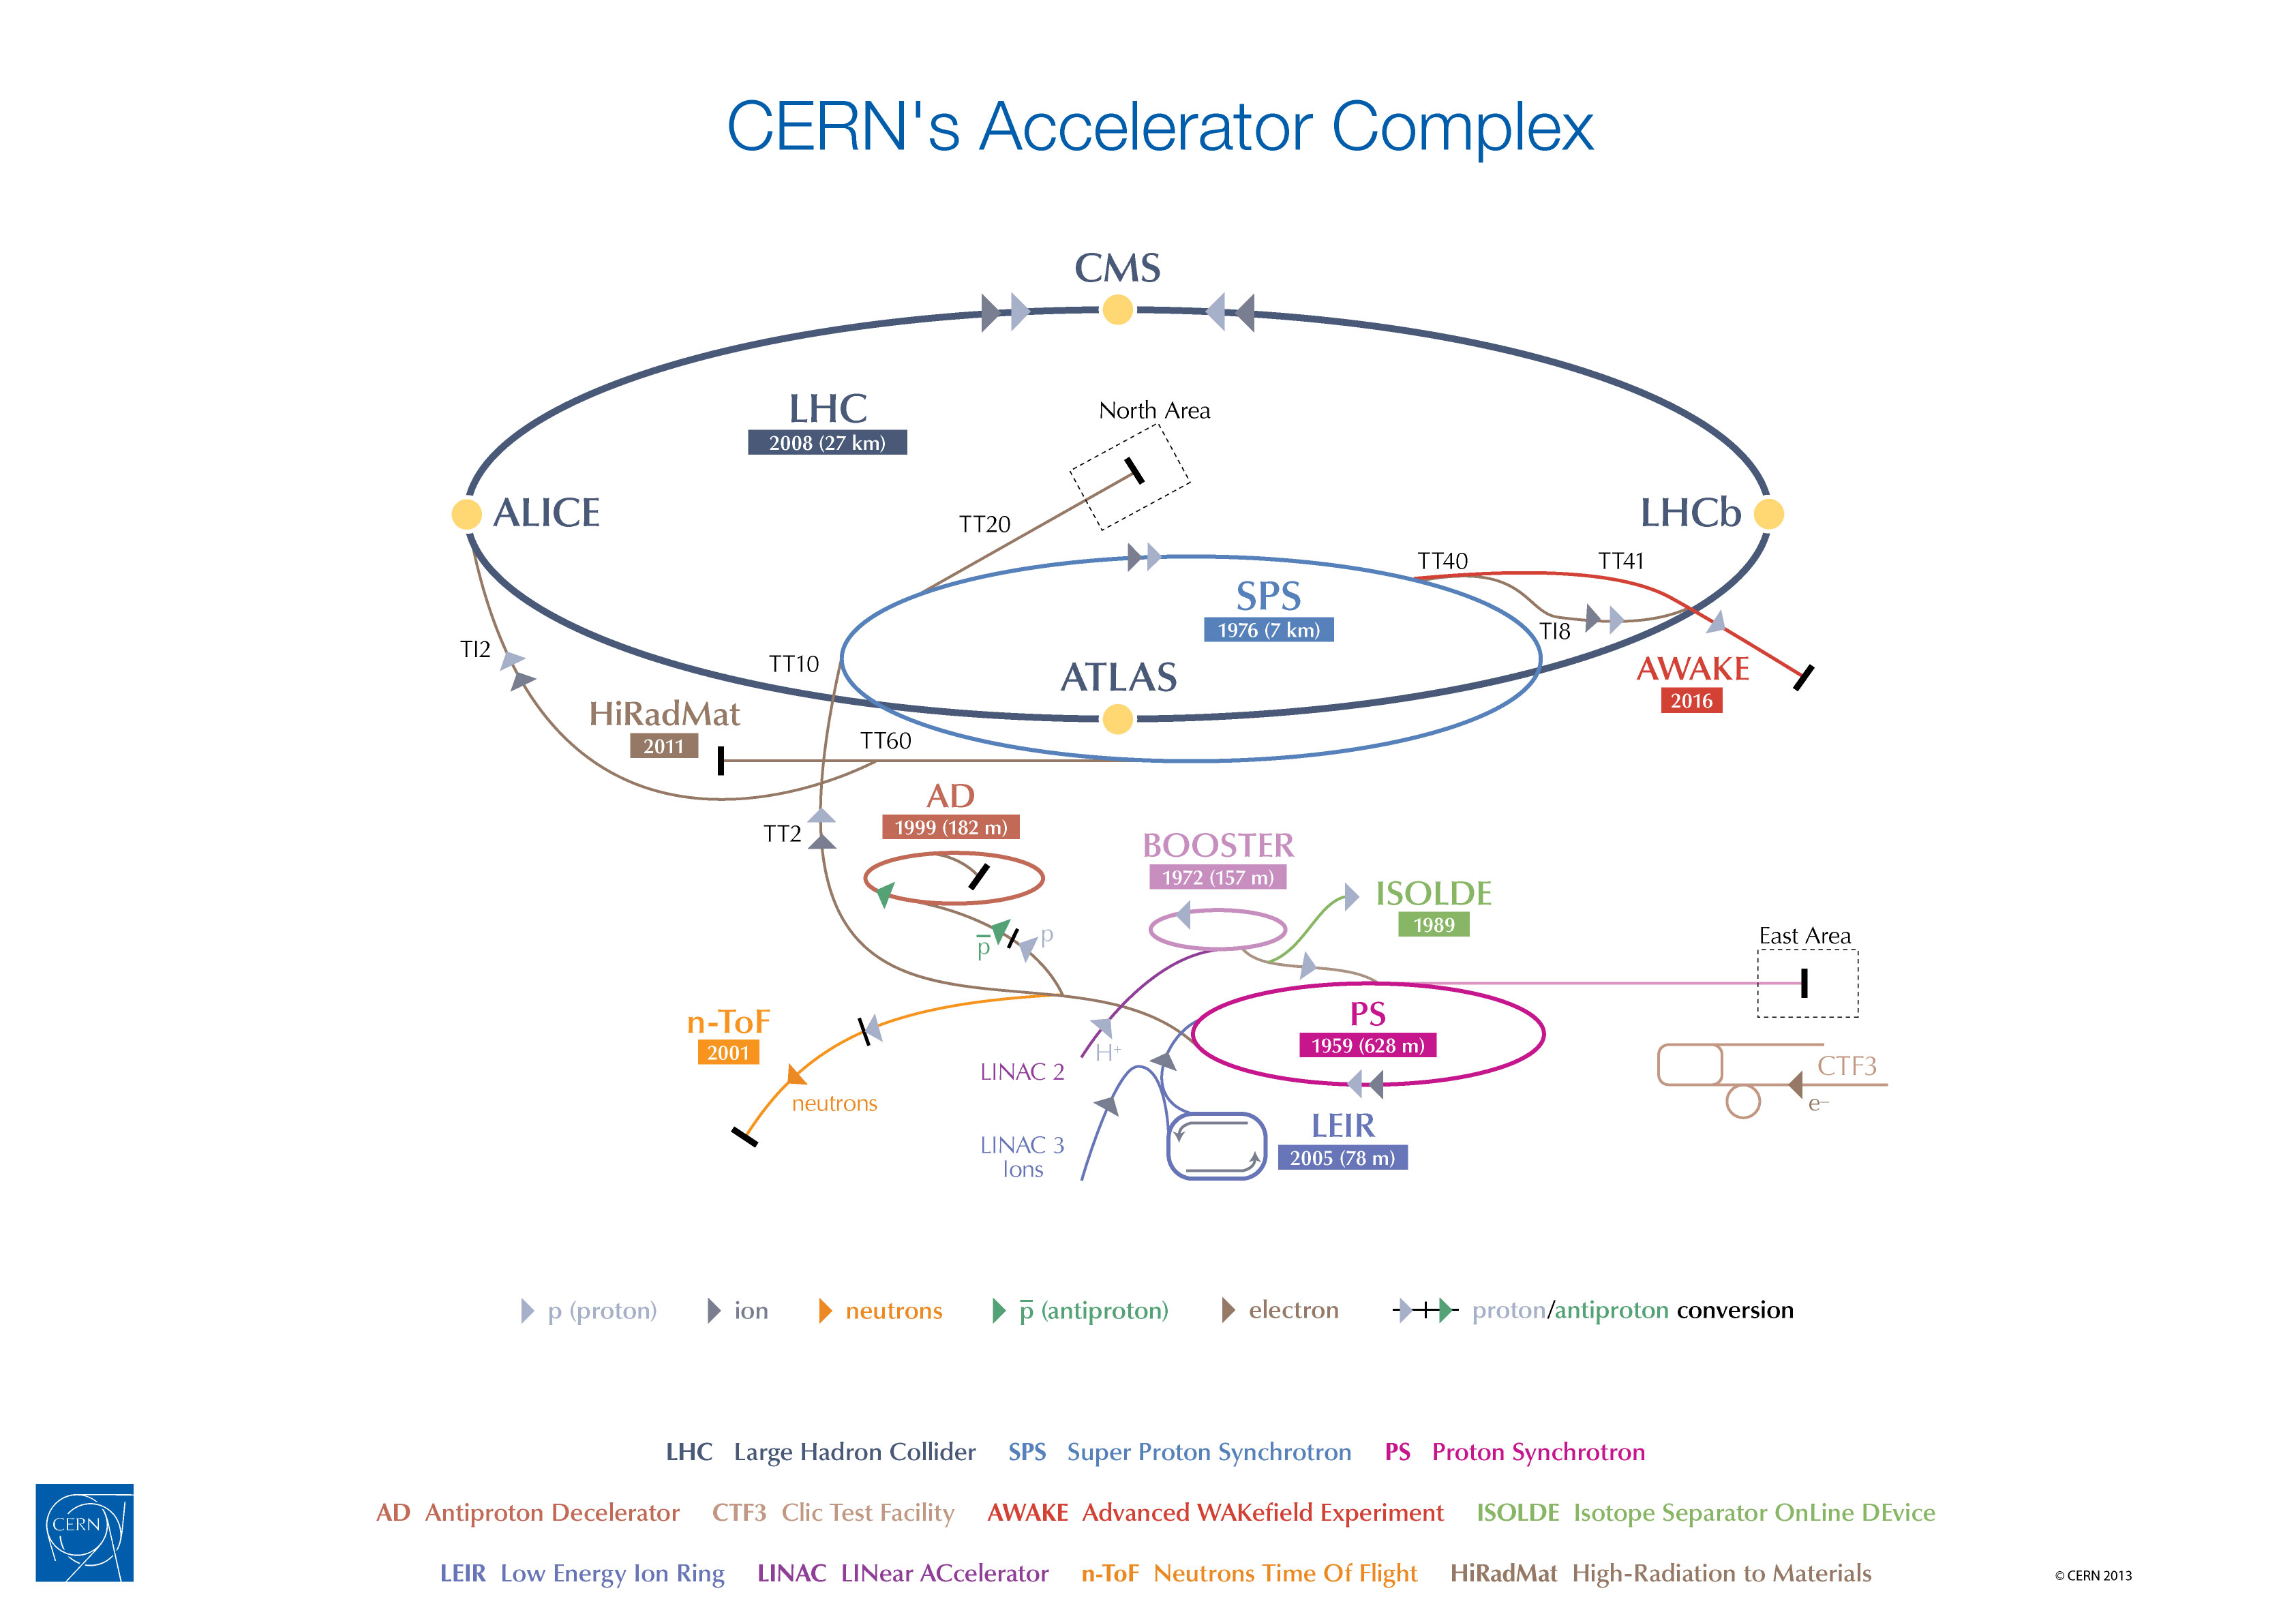
\includegraphics[width=\textwidth]{\figpath/Chapter2/CERN's-accelerator-complex2013.jpg}
		\label{fig:CERN_accelerator_complex}
	\end{subfigure}
	\begin{subfigure}[t]{0.4655\textwidth}
		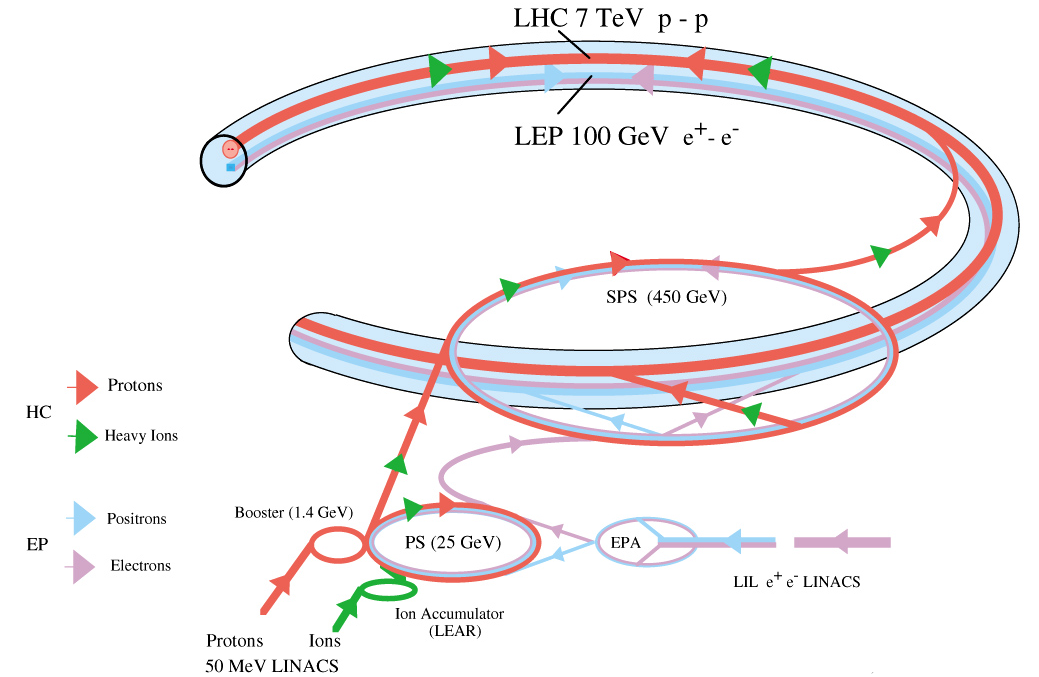
\includegraphics[width=\textwidth]{\figpath/Chapter2/lhc-pho-1993-008.png}
		\label{fig:LHC_LEP_injection_complex}
	\end{subfigure}
	\caption{Left: A schematic of the CERN accelerator complex~\cite{Marcastel:1621583}. Right: A diagram of the LHC injection chain. Also included is a diagram of the heavy ion and LEP injection chains~\cite{Jean-Luc:841568}.}
	\label{fig:CERN_accelerators}
\end{sidewaysfigure}

After being accelerated in the SPS, the proton bunches are injected into the two LHC beam pipes, which were designed to accelerate the two proton beams to $7\unit{TeV}$ (Fig~\ref{fig:LHC_beams}). Size limitations in the tunnel dictated that the the beamlines be formed by twin bore magnets. Each magnet is formed by a single mechanical structure and cryostat while containing two coils and two beam channels. The coils are made out of superconducting NbTi Rutherford cables cooled to $1.9\unit{K}$ by $120\unit{t}$ of superfluid helium. This forms the $8.33\unit{T}$ magnets necessary for beding the $7\unit{TeV}$ protons (Fig.~\ref{fig:LHC_magnet}). The LHC contains 1232 superconducting dipol magnets for bending the protons and 392 superconducting quadrupole madnets for focusing the beams. The beamline also contains sextapole, octopole, and decapole magnets, which are also used to correct and focous beams. The original LHC design calls for a bunch spacing of $25\unit{ns}$, $10^{11}$ protons per bunch, and $2808$ bunches per beam. %The acceleration is accomplished by 16 RF cavities operating at 400MHz.

\begin{figure}[!hbt]
	\centering
	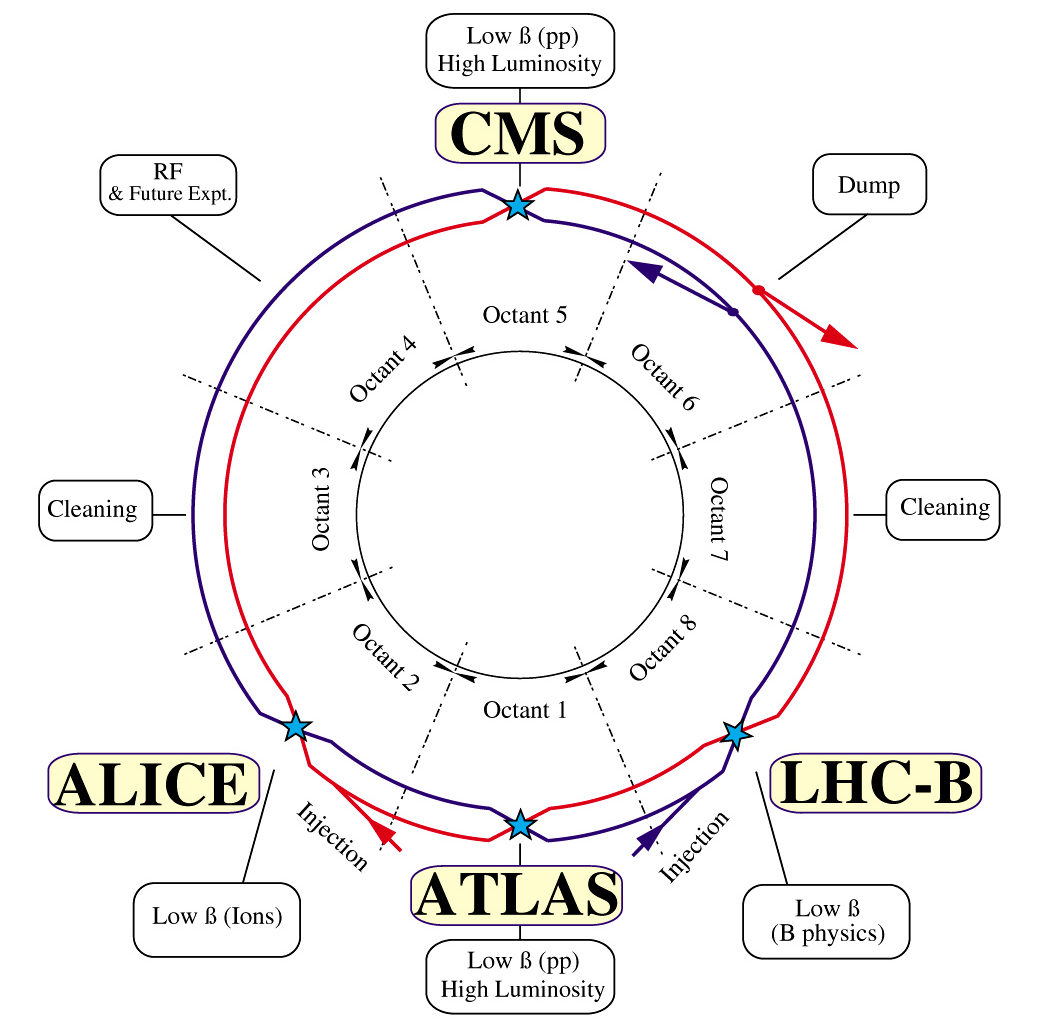
\includegraphics[width=0.95\textwidth]{\figpath/Chapter2/lhc-pho-1997-060.png}
	\caption{A diagram of the LHC beams along with the four major experiments~\cite{Jean-Luc:841573}.}
	\label{fig:LHC_beams}
\end{figure}

\begin{figure}[!hbt]
	\centering
	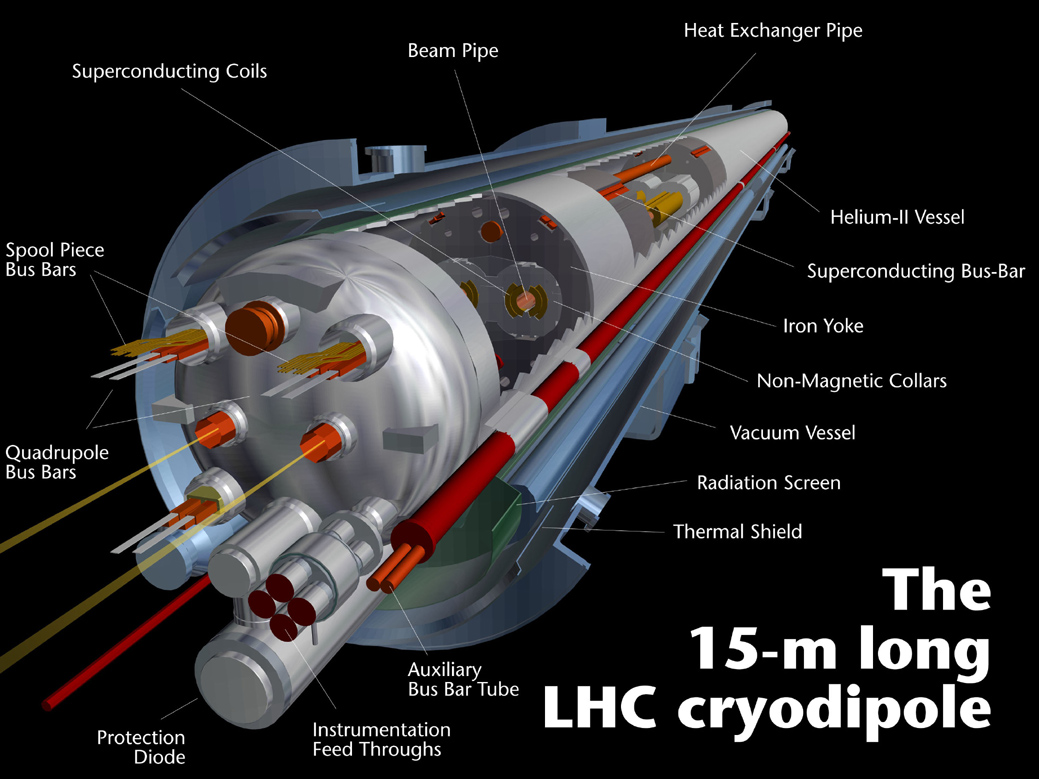
\includegraphics[width=0.95\textwidth]{\figpath/Chapter2/lhc-pho-1998-299.jpg}
	\caption{A diagram of an LHC dipole magnet and cryostat~\cite{Dailler:842253}.}
	\label{fig:LHC_magnet}
\end{figure}

The original plan was to start the LHC accelerator comple in September 2008. However, due to a catastrophic incident damaging the machine, the startup was delayed until November 23, 2009; even then colliding beams only had a center-of-mass energy of $900\unit{GeV}$. From March 30, 2010 through the end of 2011 the LHC operated with a center-of-mass energy of $7\unit{TeV}$. Then in 2012 the energy was again increased to $8\unit{TeV}$ ($4\unit{TeV}$ per beam), which is the energy of the beams during the data-taking period focused on by this thesis. It is important to note, though, that the machine has continued to operate after the 2012 data taking period and increased the center-of-mass energy to $13\unit{TeV}$ starting in 2015 (there was a planned shutdown from 2013 through early 2015).

In addition to the center-of-mass energy, collider physicists are interested in the rate at which a specific physics process occurs. This in turn is related to the cross sections, the probability that two particles will collide and react a certain way, and the luminosity. The rate of events is given by equation~\ref{eq:dn/dt}, where $\mathcal{L}$ is the collision luminosity and $\sigma$ is the cross section for a given physical process.

\begin{equation}
dN/dt=\mathcal{L}{\cdot}\sigma
\label{eq:dn/dt}
\end{equation}

The luminosity as it is described here is often called the ``instantaneous luminosity'' as this value can change from moment to moment. The ``integrated luminosity'' is then a measure of the total amount of data collected. The instantaneous luminosity itself depends upon the parameters of the LHC beams and the optical properties of the focusing system at the interaction point. This information is summed up in equation~\ref{eq:luminosity}~\cite{1742-6596-455-1-012001}:

\begin{equation}
\mathcal{L}=\frac{N^{2}n_{b}f\gamma}{4\pi\epsilon_{n}\beta^{*}}F
\label{eq:luminosity}
\end{equation}

where:

\begin{itemize}
	\item $N$: protons per bunch
	\item $n_{b}$: bunches in the LHC ring
	\item $f$: frequency of bunch revolutions around the ring 
	\item $\gamma$: relativistic factor for the protons
	\item $\epsilon_{n}$: normalized emittance of the proton beams
	\item $\beta^{*}$: beta function at the interaction point
	\item $F$: geometrical reduction factor due to the crossing angle of the beams
\end{itemize}

The maximum design luminosity of the LHC is $1{\times}10^{34}\unit{cm^{-2}s^{-1}}$. During the 2010 and 2011 run periods ($7\unit{TeV}$ center-of-mass energy) the instantaneous luminosity increased from $1{\times}10^{32}\unit{cm^{-2}s^{-1}}$ to $5{\times}10^{33}\unit{cm^{-2}s^{-1}}$. During the 2012 data-taking period, the peak instantaneous luminosity was $7.67{\times}10^{33}\unit{cm^{-2}s^{-1}}$ with a bunch spacing of $50\unit{ns}$, a maximum number of bunches of $1380$, and $\sim2.2{\times}10^{14}$ protons per beam ($\sim1.6{\times}10^{11}$ protons per bunch). The LHC delivered $23.30\unit{fb^{-1}}$ of integrated luminosity to the CMS detector of which $21.79\unit{fb^{-1}}$ was recorded. As of the end of 2016, the LHC is still running at $13\unit{TeV}$ ($6.5\unit{TeV}$ per beam) with a peak luminosity of $1.53{\times}10^{34}\unit{cm^{-2}s^{-1}}$, $2208$ bunches, and $1{\times}10^{11}$ protons per bunch~\cite{CMSWebBasedMonitoring,LumiPublic}. Figures~\ref{fig:LHC_int_lumi_pp} and~\ref{fig:LHC_lumi_per_day_pp} show the total integrated luminosity delivered by the LHC and recorded by the CMS experiment for the various data-taking periods~\cite{LumiPublic}.

\begin{figure}[!hbt]
	\centering
	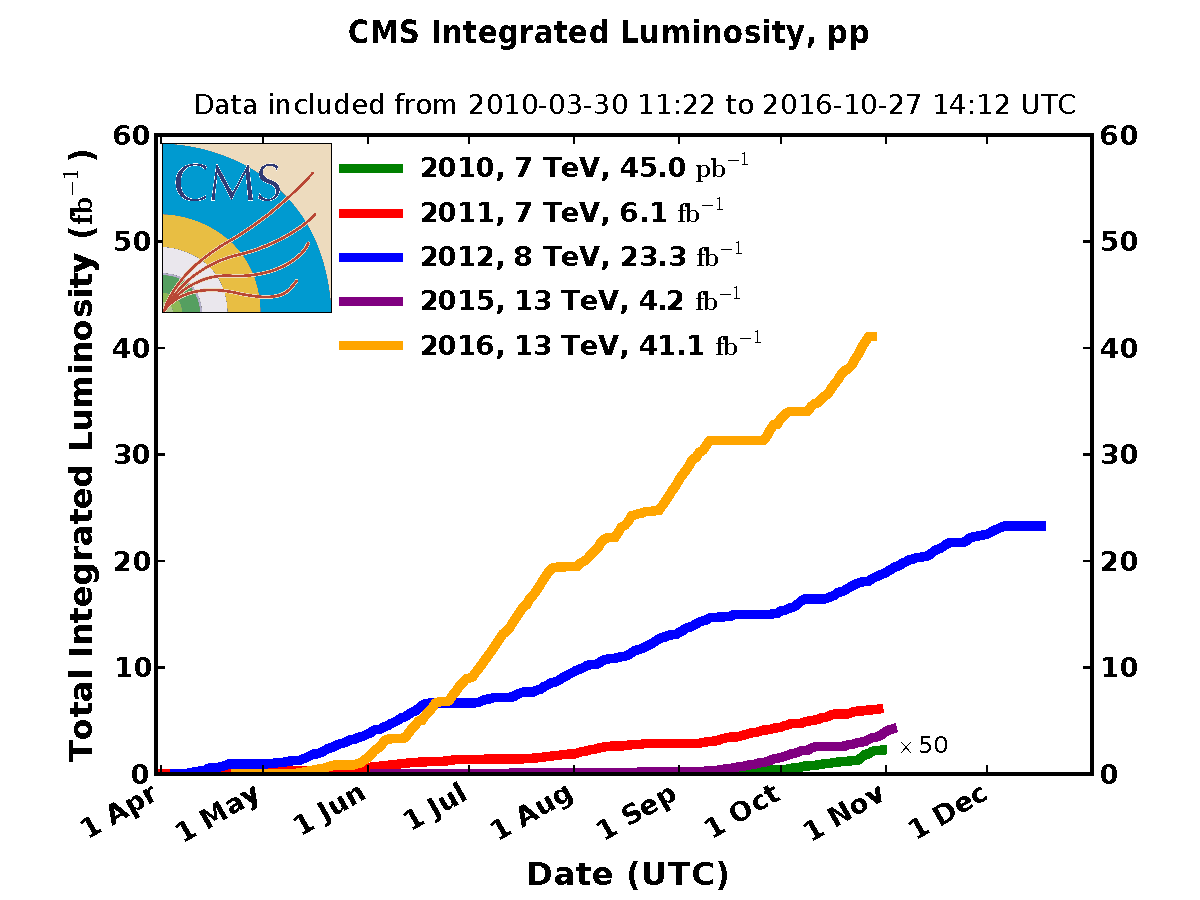
\includegraphics[width=0.95\textwidth]{\figpath/Chapter2/int_lumi_cumulative_pp_2.pdf}
	\caption{Total integrated luminosity versus time delivered to the CMS experiment for the 2010, 2011, 2012, 2015, and 2016 p-p data-taking periods~\cite{LumiPublic}.}
	\label{fig:LHC_int_lumi_pp}
\end{figure}

\begin{figure}[!hbt]
	\centering
	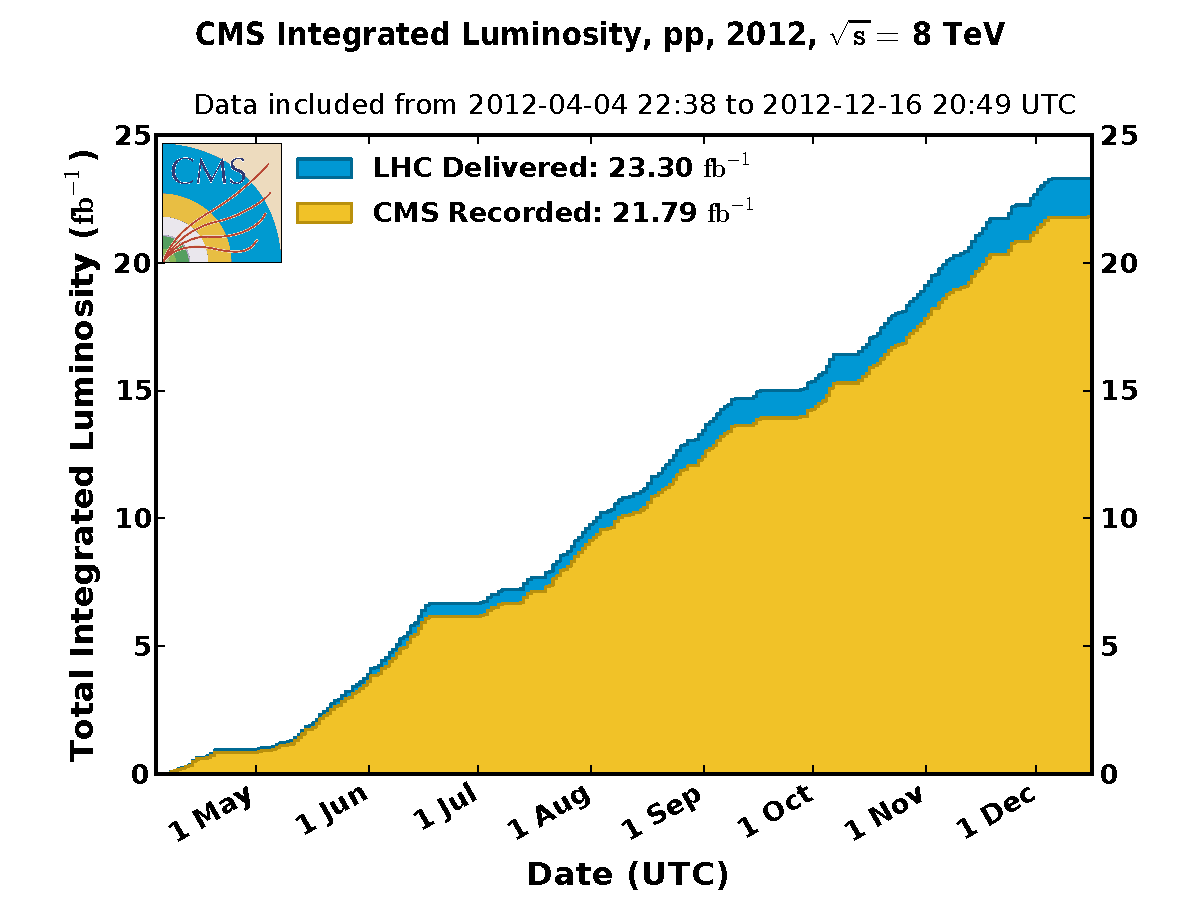
\includegraphics[width=0.95\textwidth]{\figpath/Chapter2/int_lumi_per_day_cumulative_pp_2012.pdf}
	\caption{Total integrated, offline luminosity versus day in 2012. The blue graph shows the delivered luminosity while the orange graph shows the luminosity recorded by the CMS experiment. This graph shows only the luminosity collected for p-p collisions during stable beams~\cite{LumiPublic}.}
	\label{fig:LHC_lumi_per_day_pp}
\end{figure}


\section{The CMS Detector}

TALK ABOUT THE PHYSICS GOALS?
%"The physics program of the experiment covers a wide range of goals: precision study of Standard Model processes, study of properties of the recently discovered Higgs boson, searches for physics beyond the Standard Model, and study of quark-gluon plasma." - Aysen Tatarinov

The CMS experiment is one of two general purpose detectors at the LHC; ATLAS being the other one. The detector is located $100\unit{m}$ underground near Cessy, France on the oposite side of the LHC from the main CERN site in Meyrin (see figure~\ref{fig:LHC_schematic}). It was largely built on the surface and then lowered into the collision cavern in 15 pieces, which then had to be painstakingly assembled. The detector has a cylindrical design which is $21.5\unit{m}$ in length, $15\unit{m}$ in diameter, and weights $14000$ tonnes. The shape and positioning of the detector around the interation point (IP) gives the experiment nearly $4\pi$ coverage of the proton collisions. The layout of the detector can be seen in fig.~\ref{fig:CMS_schematic}.

\begin{figure}[!hbt]
	\centering
	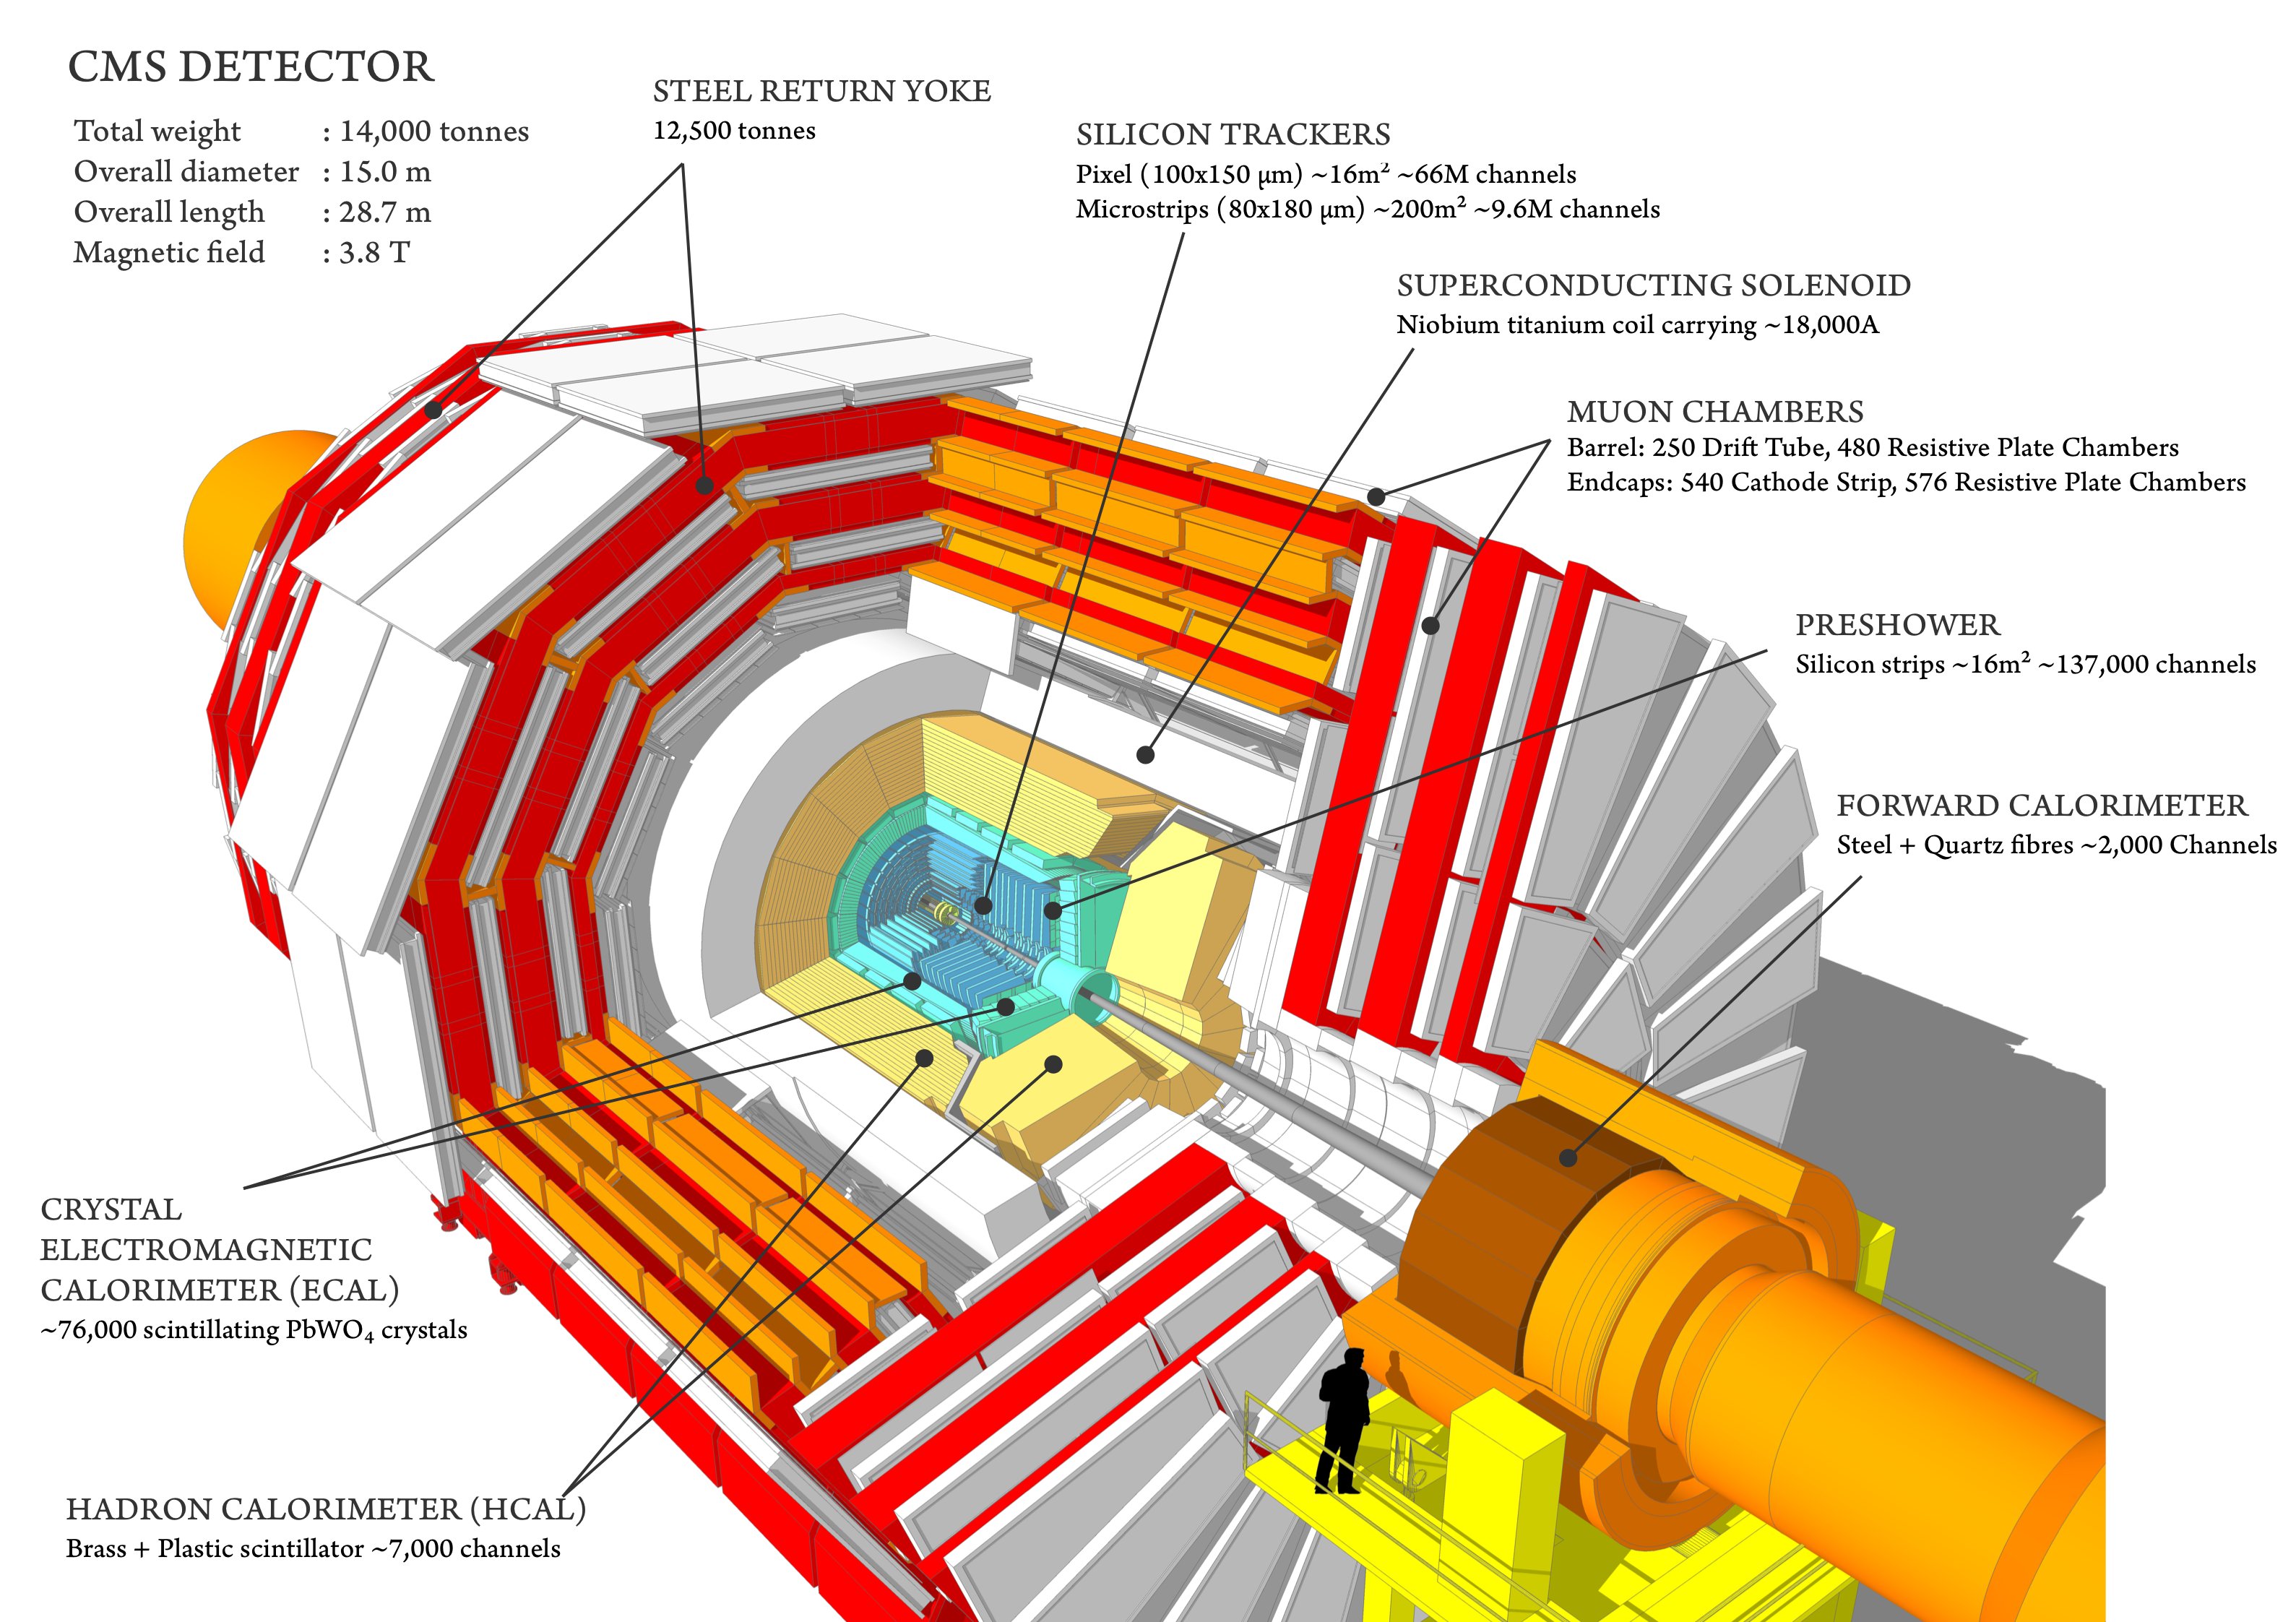
\includegraphics[width=0.95\textwidth]{\figpath/Chapter2/cms_160312_02.png}
	\caption{Schematic of the CMS detector with labels and notable figures~\cite{SketchUpCMS}.}
	\label{fig:CMS_schematic}
\end{figure}

Fig.~\ref{fig:CMS_transverse} shows how various types of particles interact within the CMS subdetectors. The following sections will describe each of the subdetectors and its properties and is based largely on Ref.~\cite{Chatrchyan:2008aa}.

\begin{figure}[!hbt]
	\centering
	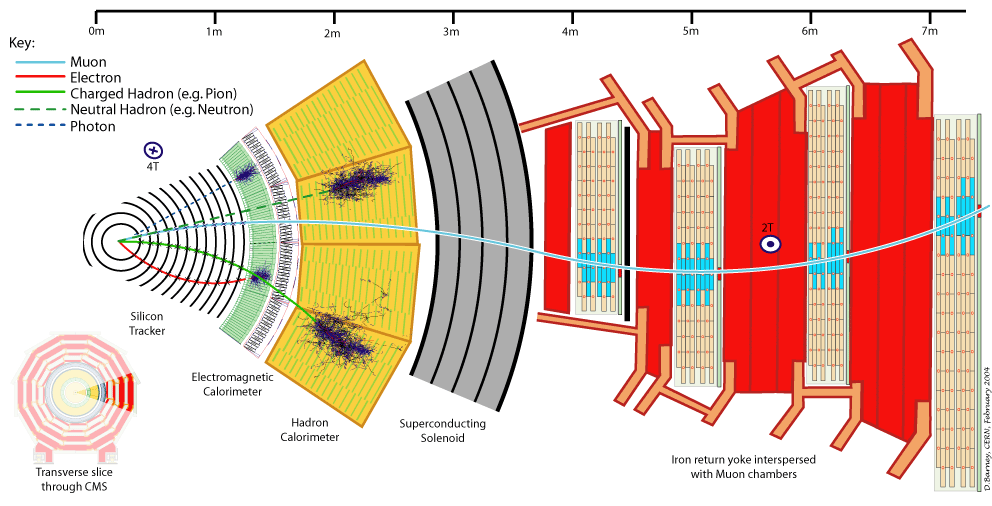
\includegraphics[width=0.95\textwidth]{\figpath/Chapter2/CMS_slice.png}
	\caption{Transverse slice of the CMS experiment with the major subdetectors and components represented. The different colored lines represent how various types of particles interact with the subdetectors~\cite{CMSSlice}.}
	\label{fig:CMS_transverse}
\end{figure}

\subsection{Coordinate System}

The IP is at the center of the detector and is the origin of the right-handed coordinate system used to describe the detector and the physics being measured (location and direction). The The z-axis is defined along the beam line with the positive 


\subsection{Tracker and Pixel Detector}
\label{sec:tracker_and_pixel}
\subsection{Electromagnetic Calorimeter}
\subsection{Hadron Calorimeter}
\label{sec:hadron_calorimeter}
\subsection{Solenoid}

The central feature of the CMS apparatus is a superconducting solenoid of 6\unit{m} internal diameter, providing a magnetic field of 3.8\unit{T}. Within the solenoid volume are a silicon pixel and strip tracker, a lead tungstate crystal electromagnetic calorimeter (ECAL), and a brass and scintillator hadron calorimeter (HCAL), each composed of a barrel and two endcap sections. Forward calorimeters extend the pseudorapidity coverage provided by the barrel and endcap detectors. Muons are measured in gas-ionization detectors embedded in the steel flux-return yoke outside the solenoid. 

\subsection{Muon System}
\subsection{Trigger}
\subsection{Luminosity Measurement}

Besides measuring the kinematics of each of the particles traversing the detector, CMS must also measure the instantaneous luminosity delivered by the LHC. Both the pixel detector (section~\ref{sec:tracker_and_pixel}) and the HF (section~\ref{sec:hadron_calorimeter}) are able to measure the luminosity to varying degrees of accuracy.

The pixel detector has a very small granularity, which means that any given pixel is activated by at most one track per bunch crossing. We can then create cluster by grouping nearby activated pixels, with the typical cluster containing an average of 5 pixels. A minimum bias event typically creates 200 clusters~\cite{CMS-PAS-LUM-12-001}. Even for events with 100 pileup interactions, a number significantly higher than was reached in 2012, the total pixel detector occupancy would only be $\sim0.1\%$. This means that the number of pixel hits should scale linearly with the number of interactions per bunch crossing, which is shown in equation~\ref{eq:pixel_luminosity_measurement}~\cite{CMS-PAS-LUM-13-001}.

\begin{equation}
\mathcal{L}=\frac{\nu<n>}{\sigma_{vis}}
\label{eq:pixel_luminosity_measurement}
\end{equation}

Here the luminosity, $\mathcal{L}$, is proportional to average number of pixel clusters, $<n>$. The other parameters are the LHC revolution frequency, $\nu=11246\unit{Hz}$ and the visible cross section, $\sigma_{vis}$, as calibrated by a Van der Meer scan~\cite{Balagura:2011yw}. In 2012 this technique was used to measure the total integrated luminosity with a systematic uncertainty of $2.6\%$.

Another method to measure the luminosity makes use of the HF, but due to some sever limitations in its accuracy, this measurement is only used as a cross-check for the pixel counting method. What makes the HF suitable for this type of measurement is that it can safely be run during unstable beams~\cite{CMS-PAS-LUM-13-001}. The average transverse energy per tower can be directly related to the luminosity or the average fraction of empty towers can be related to the mean number of interactions per crossing, which is more of in indirect measurement. The benefit of using the HF is that it can make an online determination of the luminosity within $1\unit{s}$ to an accuracy of $1\%$. One downside is that even in 2012 the levels of pileup made the luminosity relationship non-linear. Additionally, the clibration of this measurement can change due to drifts in the gains of the HF PMTs~\cite{Pedro2014}.